\documentclass[12pt,a4paper]{article}
\usepackage[utf8]{inputenc}
\usepackage[T1]{fontenc}
\usepackage{ucs}
\usepackage{amsmath}
\usepackage{amsfonts}
\usepackage{amssymb}
\usepackage{amsthm}
\usepackage{mathtools}
\usepackage[english]{babel}
\usepackage{svg}	
\usepackage{graphicx}
\usepackage{cite}
\usepackage{url}
\usepackage{color}
\usepackage{smartdiagram}
\usepackage{subfig}
\usepackage{booktabs}

\author{Martí Municoy, Alba Gordó, Jan-Hendrik Niemann\\ and Andreas Radke}
\title{Research and Innovation: Open Data}

\begin{document}
	\maketitle
	
\subsection*{Abstract}

The aim of this project is to find and visualize the events posted on \url{Meetup.com} in different cities in order to analyze the density of planned activities and to make a social study regarding most usual activities and interests. One aspect may concern different acitivities in several cities and countries. The data shall be obtained via the Meetup-API, Google Maps and a web scraping at \url{Wikipedia.org}. The most important data source for this project is the Meetup-API where we have to request the events with different Python packages like \emph{requests}. Our second task is to visualize the locations of the events on a given city map obtained by \url{googlemaps.com} or to plot different stats regarding the city events in useful charts. 

\tableofcontents
	
\section{Summary and Goals}\label{sec:summaryandgoals}
\section{Data Life-Cycle}\label{sec:datalifecycle}

%\smartdiagram[circular diagram:clockwise]{Creation, Storage, Use, Sharing, Archiving, Destruction}

In the following section we have a closer look at the terms "data lifecycle" and "data lifecycle management".\\"Data lifecycle" is a term which tries to describe the life of data and information. Since there is no unique definition of a data lifecycle, we define the folloing six stages: creation, storage, use, sharing, archiving and destruction \cite{spirion}.

\begin{enumerate}
	\item \textbf{Creation}: Data is created. It can be created as a structured or unstructured set of data, can be obtained by collection, measurements, generated or gathered. We create our data by using the \textcolor{red}{request-API}. During pur process we gather the needed data from the \url{Meetup.com} website. By performing a web scraping at \url{Wikipedia.org} we gather the number of population for different cities and its districts. In this way we create our data which is needed for this project.
	\item \textbf{Storage}: Once the data is created it has to be stored. Depending on the purpose there are different kinds of storage solutions. However, this is not subject of this report. In our case both the data gathered from \url{Meetup.com} and \url{Wikipedia.org} is saved a csv-files on the hard drive.
	\item \textbf{Use}: Data can be viewed, modified analyzed, corrected, interpreted, visualized, joined,... We use our data the visualize the behaviour of cities. We join our data from different sources and visualize it on a given map which can be seen as data as well. After visualizing the data we interpret the newly created data to obtain information about the cities.
	\item \textbf{Sharing}: Data can be shared. There are several ways of sharing like sharing with persons, applications or in different operating environments. Since our data is not shared during the the process, we are not explaining this stage of the data lifecycle in detail.
	\item \textbf{Archiving}: When the data leaves the active use, one should archive it in a suitable way. Since archiving is very similar to storaging, one can use the same methods. One difference may be that saved data needs to be compressed to save storage or protected to prevent unwanted changed. Therefore, the access is slightly more difficult than for data in active use. For this project we save our data on the one hand as GeoJSON-files and on the other hand as csv-files. Whereas the data saved in the GeoJSON-files are not subject to changes, since the geopolitical structure of cities does not change during this project, the csv-files underlie changes. For this reason there is a last stage in the data lifecycle.
	\item \textbf{Destruction}: There are several reasons why one should destroy data. On the one hand the volume of archived data increases and one needs to save storage to store new data. On the other hand the data gets old and is not needed anymore. It is not up to date and can be replaced by newer versions. The second case is applicable for our work. During every single run of the program new csv-files with event data and new csv-files containing populations data are created. Especially the event data underlie a rapid change.
\end{enumerate}

The term "data lifecycle management" describes the process that helps to organize the flow of data throughout its lifecycle.
\section{Tools and Data}\label{sec:toolsanddata}
The main work for our project was done in the Python programming language in version 3.6 \cite{python}. \cite{gmaps},  \cite{matplotlib} \cite{jupyter}, \cite{requests}

\section{Results}\label{sec:results}

To draw meaningful conclusions we created several types of visualization of the data. First and foremost we plotted the open events onto a map - either as a point map, e.g Figure \ref{fig:barcelonapoints}, or as a occurrences distribution map for each city district, e.g. Figure \ref{fig:barcelonamap}. Additionally numerous bar charts were created with the number of categories (absolute and per capita) per city, compare Figure \ref{fig:barcelonabar}, and vice versa. 

In this chapter we will shortly discuss several cities and their interesting characteristics. 

\begin{figure}[!htp]
	\includegraphics[width=1\linewidth]{images/Barcelona_points.png}
	\caption{Snippet of Barcelona with Open Events}\label{fig:barcelonapoints}	
\end{figure}

\begin{figure}[!htp]
	\includegraphics[width=1\linewidth]{images/Barcelona_points_Language.png}
	\caption{Snippet of Barcelona with only Language \& Ethnic Identity Events}\label{fig:barcelonapointslanguage}	
\end{figure}

\begin{figure}[!htp]
	\includegraphics[width=1\linewidth]{../plotting/pngs/categories/Barcelona.png}
	\caption{Activities per Category in Barcelona}\label{fig:barcelonabar}	
\end{figure}

\subsection*{Barcelona}

In Figure \ref{fig:barcelonapoints} one can see an example of Barcelona with open events plotted as points. The different colors represent different Meetup categories. One can see that there are slightly more green points which represent the Meetup category \emph{Language and Ethnic Identity}. A more specific view offers Figure \ref{fig:barcelonapointslanguage} with only the points corresponding to this specific category. Furthermore the already mentioned Chart \ref{fig:barcelonabar} shows that the Language and Ethnic Identity events are indeed the most frequent category which may be an indicator for the diverse and multi-cultural Catalan capital. 

\begin{figure}[!htp]
	% Maximum length
	\subfloat[Activity per District]{\label{fig1:a}\includegraphics[width=0.49\linewidth]{images/activities_of_districts/Barcelona.png}}\hfill
	\subfloat[Activity per Capita per District]{\label{fig1:b}\includegraphics[width=0.49\linewidth]{images/activities_per_capita_of_districts/Barcelona.png}}%
	\caption{Barcelona}\label{fig:barcelonamap}
\end{figure}

The most activities are unsurprisingly in the populous Eixample district but per inhabitant there are more events in Ciutat Vella. Despite having a natural concentration in more centric areas for Barcelona it seems that the activities are a bit more spread out to the whole city. This can be due to Barcelonas small size and its high population density. 
In contrast there are Marid-Centro (Figure \ref{fig:madridmap}), New York-Manhattan (\ref{fig:newyorkmap}) and Hong Kong (\ref{fig:hongkongmap}) where the open events are strongly concentrated in one or a few central districts. 

\subsection*{London}

London seems rather centric with Westminster as the hot-spot district. But especially per capita everything is overshadowed by the small and little populated City of London. Later we will see that London has the highest number of events outside of Europe (in our dataset). 

The most popular categories are Socializing and Tech. 

\begin{figure}[!htp]
	% Maximum length
	\subfloat[Activity per District]{\label{fig1:a}\includegraphics[width=0.49\linewidth]{images/activities_of_districts/London.png}}\hfill
	\subfloat[Activity per Capita per District]{\label{fig1:b}\includegraphics[width=0.49\linewidth]{images/activities_per_capita_of_districts/London.png}}%
	\caption{London}
\end{figure}


\subsection*{Berlin}

Because of the historical division of Berlin it does not have one big city center. One can see (Figure \ref{fig:berlinpoints}) that event concentration is slightly shifted to the east around Prenzlauer Berg (south of Pankow, East of Mitte and Friedrichshain-Kreuzberg. In contrast there is only a smaller focus at the City West (Zoologischer Garten, Charlottenburg-Wilmersdorf). 

\begin{figure}[!htp]
	% Maximum length
	\subfloat[Activity per District]{\label{fig1:a}\includegraphics[width=0.49\linewidth]{images/activities_of_districts/Berlin.png}}\hfill
	\subfloat[Activity per Capita per District]{\label{fig1:b}\includegraphics[width=0.49\linewidth]{images/activities_per_capita_of_districts/Berlin.png}}%
	\caption{Berlin}
\end{figure}


\begin{figure}[!htp]
	\includegraphics[width=1\linewidth]{images/Berlin_points.png}
	\caption{Snippet of Berlin with Open Events}\label{fig:berlinpoints}	
\end{figure}

Regarding the categories (\ref{fig:berlinbar}) it is obvious that the \emph{Tech} activities dominate in Berlin. The reason for this increased interest in technology may be due to a high number of upcoming startups. 
But actually the high dominance (three times larger than the second favorite; largest dominance) of technology events in contrast to other categories is a trait which all three examined German cities share. One conclusion would that Meetup seems so far to be limited to \emph{tech-interested} people in Germany. 

\begin{figure}[!htp]
	\includegraphics[width=1\linewidth]{../plotting/pngs/categories/Berlin.png}
	\caption{Activities per Category in Berlin}\label{fig:berlinbar}	
\end{figure}


\subsection*{Madrid}

Almost all events are concentrated in Madrid-Centro. Madrid's most favorite categories are by far Tech and Languages \& Ethnic Identity. 

\begin{figure}[!htp]
	% Maximum length
	\subfloat[Activity per District]{\label{fig1:a}\includegraphics[width=0.49\linewidth]{images/activities_of_districts/Madrid.png}}\hfill
	\subfloat[Activity per Capita per District]{\label{fig1:b}\includegraphics[width=0.49\linewidth]{images/activities_per_capita_of_districts/Madrid.png}}%
	\caption{Madrid}
\end{figure}

\subsection*{Paris}

Paris is an example for a more evenly distributed city - at least in the total number of events per district. This may be due to its small size and dense population (compare Barcelona). The picture would probably be different if one considers the vast metropolitan area of Paris with its 12 Mio. people and its area of 17000 $ km^2 $ (in contrast to the actual 2.2 Mio. and 105 $ km^2 $)
Again Tech and Language and Ethnic Identity are the most favored categories. 

\begin{figure}[!htp]
	% Maximum length
	\subfloat[Activity per District]{\label{fig1:a}\includegraphics[width=0.49\linewidth]{images/activities_of_districts/Paris.png}}\hfill
	\subfloat[Activity per Capita per District]{\label{fig1:b}\includegraphics[width=0.49\linewidth]{images/activities_per_capita_of_districts/Paris.png}}%
	\caption{Paris}
\end{figure}


\subsection*{Brussels}

In this case we actually did not consider the City of Brussels but rather the Brussels-Capital Region. But one can clearly see the bright yellow shape which represents the City of Brussels (this is one \emph{district}!). Per capita some central regions like Ixelles show a higher activity too. 
\begin{figure}[!htp]
	% Maximum length
	\subfloat[Activity per District]{\label{fig1:a}\includegraphics[width=0.49\linewidth]{images/activities_of_districts/Brussels.png}}\hfill
	\subfloat[Activity per Capita per District]{\label{fig1:b}\includegraphics[width=0.49\linewidth]{images/activities_per_capita_of_districts/Brussels.png}}%
	\caption{Brussels}\label{fig:madridmap}
\end{figure}

\subsection*{Hamburg}
Hamburg is the second biggest city in Germany. As in Berlin mostly tech-interested people are using \url{Meetup.com}. Looking at the figures one can clearly identify the trending districts in Hamburg which are "Hamburg-Mitte" (middle), "Altona", "Eimsbüttel" and "Hamburg-Nord" (from west to east). One reason for this might be that lots of young people are living in these districts. For example, in "Hamburg-Mitte" there is the very famous "St. Pauli". In this part of the district a great part of the nightlife take place. Other districts like "Altona" and "Eimsbüttel" are trending as well since the University of Hamburg is located in "Rotherbaum" which is a part of "Eimsbüttel and close to "Altona", "Hamburg-Mitte" and "Hamburg-Nord".

\begin{figure}[!htp]
	% Maximum length
	\subfloat[Activity per District]{\label{fig1:a}\includegraphics[width=0.49\linewidth]{images/activities_of_districts/Hamburg.png}}\hfill
	\subfloat[Activity per Capita per District]{\label{fig1:b}\includegraphics[width=0.49\linewidth]{images/activities_per_capita_of_districts/Hamburg.png}}%
	\caption{Hamburg}
\end{figure}

\subsection*{New York City}

The biggest city of the United States of America has the second largest amount of open events in our dataset. Here it is necessary to keep in mind that the real number of events can vary if the Meetup communities are more organized in closed groups. 

The picture New York shows is as one would expect. At least in the case for Manhattan which is by far \emph{the} center of the City with over 1000 open events. It is followed by the distant second Brooklyn less than one third of activities. Staten Island and the Bronx are hardly active. 

\begin{figure}[!htp]
	% Maximum length
	\subfloat[Activity per District]{\label{fig1:a}\includegraphics[width=0.49\linewidth]{images/activities_of_districts/NewYork.png}}\hfill
	\subfloat[Activity per Capita per District]{\label{fig1:b}\includegraphics[width=0.49\linewidth]{images/activities_per_capita_of_districts/NewYork.png}}%
	\caption{New York City}\label{fig:newyorkmap}
\end{figure}

As \emph{Meetup Inc.} is based in New York it shows a diverse picture in regards to categories. The leading categories are Sports and Recreation, Tech, Career and Business and Socializing. 

\subsection*{Munich}

As the third German city in our set Munich does not seem to be much different than Berlin and Hamburg. Again most Meetup members are interested in Technology. In total number of activities Munich beats the more populated Hamburg and even Berlin if one considers activities per inhabitant. 

\begin{figure}[!htp]
	% Maximum length
	\subfloat[Activity per District]{\label{fig1:a}\includegraphics[width=0.49\linewidth]{images/activities_of_districts/Munich.png}}\hfill
	\subfloat[Activity per Capita per District]{\label{fig1:b}\includegraphics[width=0.49\linewidth]{images/activities_per_capita_of_districts/Munich.png}}%
	\caption{Munich}
\end{figure}

\subsection*{Hong Kong}

The first thing we notice is that Hong Kong has the lowest number of activities per capita in our dataset (compare Figure \ref{fig:categories_all_percapita}). It seems that \url{Meetup.com} did not reach Hong Kong and maybe the whole Chinese or even Asian market. 
As a business center it shows the largest activity in Socializing and Career and Business followed by Sports and Recreation. 

\begin{figure}[!htp]
	% Maximum length
	\subfloat[Activity per District]{\label{fig1:a}\includegraphics[width=0.49\linewidth]{images/activities_of_districts/HongKong.png}}\hfill
	\subfloat[Activity per Capita per District]{\label{fig1:b}\includegraphics[width=0.49\linewidth]{images/activities_per_capita_of_districts/HongKong.png}}%
	\caption{Hong Kong}\label{fig:hongkongmap}
\end{figure}


\begin{figure}[!htp]
	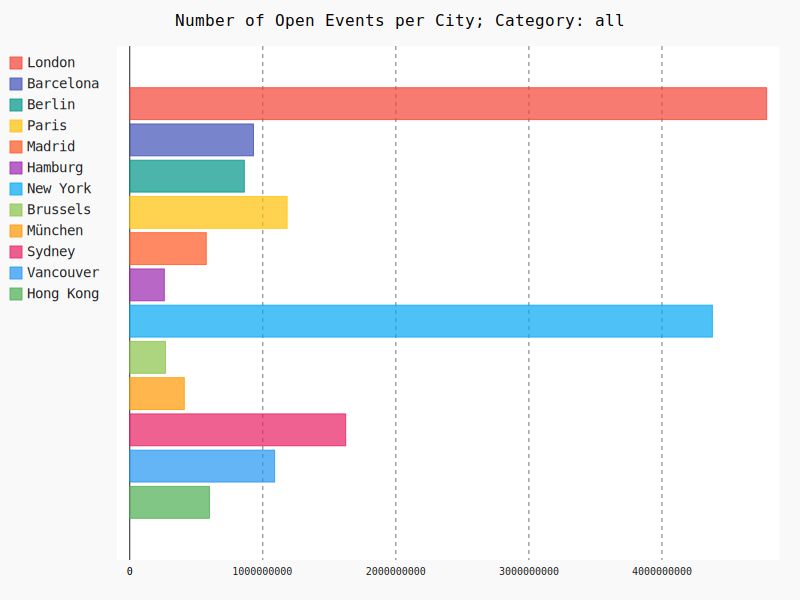
\includegraphics[width=1\linewidth]{../plotting/pngs/activities_per_city_per_capita/all.png}
	\caption{Number of Open Events in all Categories per Capita}\label{fig:categories_all_percapita}	
\end{figure}

\section{Legal and Ethical Issues}\label{sec:legalandethicalissues}


The privacy policy of a work must be at least as protective of the information as the most restrictive of the sources used. As a matter of fact, all the data sources used along the work need to be taken into account in the study of its legal and ethical issues.

The issues related with data protection copyright and intellectual property legislation can be very tedious, specially if the source is a private company. To enhance the understanding, and even though some of the sources do not present copyright-licenses of this type, the icons used and released by the non-profit organisation Creative Commons will be used in this section. The Creative Commons licenses  require attribution for copying, sharing and verbatim uses but there are other restrictions that may apply (see Table \ref{table_5}).

\begin{table}[]
\centering
\caption{ The four types of restrictions that may apply to a Creative Common license.}
\label{table_5}
\begin{tabular}{ p{1cm} p{1cm} p{10cm}}
    \begin{minipage}{.1\textwidth}
      \includegraphics[scale=.07]{images/cc_by.png}
    \end{minipage} & \textbf{BY} & \textbf{Attribution} - credit to the creator is required                                                                                                             
    \\
 \begin{minipage}{.1\textwidth}
      \includegraphics[scale=.07]{images/cc_sa.png}
    \end{minipage} & \textbf{SA} & \textbf{Share Alike} - distribution of the work needs to be under the same licence of the work (e.g. a copy made from a Creative Commons work cannot be copyrighted) 
    \\
 \begin{minipage}{.1\textwidth}
      \includegraphics[scale=.07]{images/cc_nd.png}
    \end{minipage} & \textbf{ND} & \textbf{No Derivatives} - cannot make changes to or remix the work                                                                                                    \\
 \begin{minipage}{.1\textwidth}
      \includegraphics[scale=.07]{images/cc_nc.png}
    \end{minipage} & \textbf{NC} & \textbf{Non-commercial} - commercial use of the work is not permitted                                                                                               
\end{tabular}
\end{table}

\subsection{Meetup API}

The information regarding the use that can be done with any information extracted from the Meetup API is detailed in 5.8 \textit{API License} of the \textit{Terms of Service} section and expanded in the some other sections to which a link is attached. The introduction of the subsection is attached as follows. From this paragraph (and from the rest of the section), it is clear that restrictions \textbf{BY}, \textbf{SA}, \textbf{ND} apply.

\vspace{0.5cm}
"Meetup grants to you a limited, non-exclusive, non-transferable, non-sublicensable, revocable license to use the Meetup application programming interface, including data or other Content made available via the Meetup API, (...) solely to facilitate the development of event and group related applications using Platform data and developer tools."
\vspace{0.5cm}

Notice however that commercial use of the work is not said to be prohibited. Section \textit{Meetup API License Guidelines} details what kind of applications and under what conditions (i.e., "enhance the Meetup experience or create specialized versions") the commercial use of the information provided by this platform is allowed. Not surprisingly, though, the conditions given already restrict a lot the possibility of making any commercial use of the data, so restriction \textbf{NC} could almost be added to the restrictions list too.

\subsection{Google Maps API}

The restrictions in the use of this API are considerably more complicated than the ones in the Meetup case, and are spread out in sections 6 to 12 of the \textit{Google Maps/Google Earth APIs Terms of Service}. The summary of restrictions is found in section 8.2, \textit{Service License}, where it is made clear that the license to use the Service is non-sublicensable. A part from some restrictions, section 9.1 \textit{.1 Free, Public Accessibility to Your Maps API Implementation.} specifies the terms under which a commercial use of the Service would be allowed. Attribution and non derivatives restrictions are also specified in sections 9.4 and 10.5 respectively, so the whole set of restrictions is finally  \textbf{BY}, \textbf{SA}, \textbf{ND} and \textbf{NC} in some cases.

\subsection{Different sources of \textit{.geoJSON} files}



\subsection{Wikipedia}

As explained in the \textit{Terms} section of Wikimedia, the contents of this platform are only restricted by \textbf{BY} and \textbf{SA}.

\section{Limitations and Future Work}\label{sec:limitationsandfuturework}

One major issue is that this project is depending strongly on the quality of the data available at \url{Meetup.com}. We have to rely on the users of \url{Meetup.com} so this issue can hardly be improved. One idea would be to integrate other social services like \url{Facebook.com} to extrend our data source and to get more independent. In this way one could also fix the problem that \url{Meetup.com} might be less known in non-English speaking countries. Having a wide base as data source one gets more independent of local and regional preferences regarding the social networks.\\Another problem is that this project has the potential to be extended in the following way: So far our program is restricted to predefined cities. It is not possible to select new cities or regions. This is due to the fact that we work with GeoJSON-files which are saved locally on the hard drive. \textcolor{red}{The second problem is that some Wikipedia pages for the cities are not coherent so that one needs to be careful}. One improvement could be to create a user interface and the possibility to select new cities and regions. By selecting single categories of events one could get special information, e.g. where to go running. Additional, in an application, one could automatically create suitable graphics, charts and tables.\\Another limitation is as well related to \url{Meetup.com}. Since we only have one data source for events, we only can give sufficient criterions for districts. A district having lots of events seems to be trening. However, a district having less events is not automatically less interesting and popular. It just means that its inhabitants are not using \url{Meetup.com}. Again, one should take more data sources into account.

Our tool could help social scientists to provide theire hypothesis with proving data. Beside literature, studies and surveys our tool seems to be a good method for analyzing the behaviour and preferences of populations.

\section*{Appendix}\label{sec:appendix}

\subsection*{Sources of GeoJSON Files}	
%\csvautotabular{geojson.csv}

\newpage

\bibliography{bibliography}{}
\bibliographystyle{plain}
\end{document}